\documentclass[10pt,journal,compsoc]{IEEEtran}
\usepackage[spanish]{babel}
\usepackage{listings}
% Just add \input{smalltalkEnv} to your file
% then you can use :
% \begin{lstlisting}[language=Smalltalk]
% false become: true.
% \end{lstlisting}

\usepackage{color}
\usepackage{listings}
\usepackage{etoolbox}

\definecolor{stComment}{rgb}{0.5,0.5,0.5}
\definecolor{stString}{rgb}{0.58,0,0.82}
\definecolor{stKeywords}{rgb}{0.21,0.55,0.7}
\definecolor{stNumbers}{rgb}{.5,0,0}

\newtoggle{InString}{}% Keep track of if we are within a string
\togglefalse{InString}% Assume not initally in string
\newcommand*{\ColorIfNotInString}[1]{\iftoggle{InString}{#1}{\color{stNumbers}#1}}%
\newcommand*{\ProcessQuote}[1]{#1\iftoggle{InString}{\global\togglefalse{InString}}{\global\toggletrue{InString}}}%

\lstdefinelanguage{Smalltalk}{
	keywordstyle=\color{stKeywords},
	commentstyle=\color{stComment},
	stringstyle=\color{stString},
	alsoletter=\#,
	identifierstyle=\idstyle, 
	showstringspaces=false,
	morekeywords={true,false,self,super,nil},
	sensitive=true, 
	morecomment=[s]{"}{"}, 
	morestring=[d]', 
	style=SmalltalkStyle,
	tabsize=2,
}


\makeatletter%
\newcommand*\idstyle[1]{%
	\expandafter\id@style\the\lst@token{#1}\relax%
}
\def\id@style#1#2\relax{%
	\ifnum\pdfstrcmp{#1}{\#}=0%
	\ttfamily\color{stString} \the\lst@token%
	\else%
	\edef\tempa{\uccode`#1}%
	\edef\tempb{`#1}%
	\ifnum\tempa=\tempb%
	\ttfamily\color{blue} \the\lst@token%
	\else%
	\the\lst@token%
	\fi%
	\fi%
}

\lstdefinestyle{SmalltalkStyle}{ 
	literate=%
	{^}{{$\uparrow$}}1% 
	% {"}{{{\ProcessQuote{"}}}}1% Disable coloring within double quotes
	% {'}{{{\ProcessQuote{'}}}}1% Disable coloring within single quote
	{0}{{{\ColorIfNotInString{0}}}}1%
	{1}{{{\ColorIfNotInString{1}}}}1%
	{2}{{{\ColorIfNotInString{2}}}}1%
	{3}{{{\ColorIfNotInString{3}}}}1%
	{4}{{{\ColorIfNotInString{4}}}}1%
	{5}{{{\ColorIfNotInString{5}}}}1%
	{6}{{{\ColorIfNotInString{6}}}}1%
	{7}{{{\ColorIfNotInString{7}}}}1%
	{8}{{{\ColorIfNotInString{8}}}}1%
	{9}{{{\ColorIfNotInString{9}}}}1%
} 
\usepackage{graphicx}
\usepackage{wrapfig}
\usepackage{lipsum}
\ifCLASSOPTIONcompsoc
  \usepackage[nocompress]{cite}
\else
  \usepackage{cite}
\fi

\ifCLASSINFOpdf
\else
\fi
\newcommand\MYhyperrefoptions{=true,bookmarksnumbered=true,
pdfpagemode={UseOutlines},plainpages=false,pdfpagelabebookmarksls=true,
colorlinks=true,linkcolor={black},citecolor={black},urlcolor={black},
pdftitle={Smalltalk},
pdfsubject={Lenguaje de Progemaci\'on Smalltalk},
pdfauthor={Daniel, Wilbert, Anthony, Bryan},
}
\renewcommand{\lstlistingname}{Cuadro}
\lstset{
	extendedchars=true,
	frame = single, 
	language=Modula-2, 
	framexleftmargin=3pt
}
\hyphenation{op-tical net-works semi-conduc-tor}


\begin{document}
\title{Smalltalk}

\author{Daniel~Delgado,~\IEEEmembership{Estudiante,~ITCR,}
	Wilbert~Gonzales,~\IEEEmembership{Estudiante,~ITCR,}
	Anthony~Leandro,~\IEEEmembership{Estudiante,~ITCR,}
	and~Bryan~Mena,~\IEEEmembership{Estudiante,~ITCR}
}
\markboth{Lenguajes de Programaci\'on, Tarea Corta 8, Noviembre 2017}
{Shell \MakeLowercase{\textit{et al.}}: \LaTex}


\maketitle

\IEEEdisplaynontitleabstractindextext

\IEEEpeerreviewmaketitle

\section{Datos Historicos}
\begin{wrapfigure}{R}{0.3\textwidth}
	\centering
	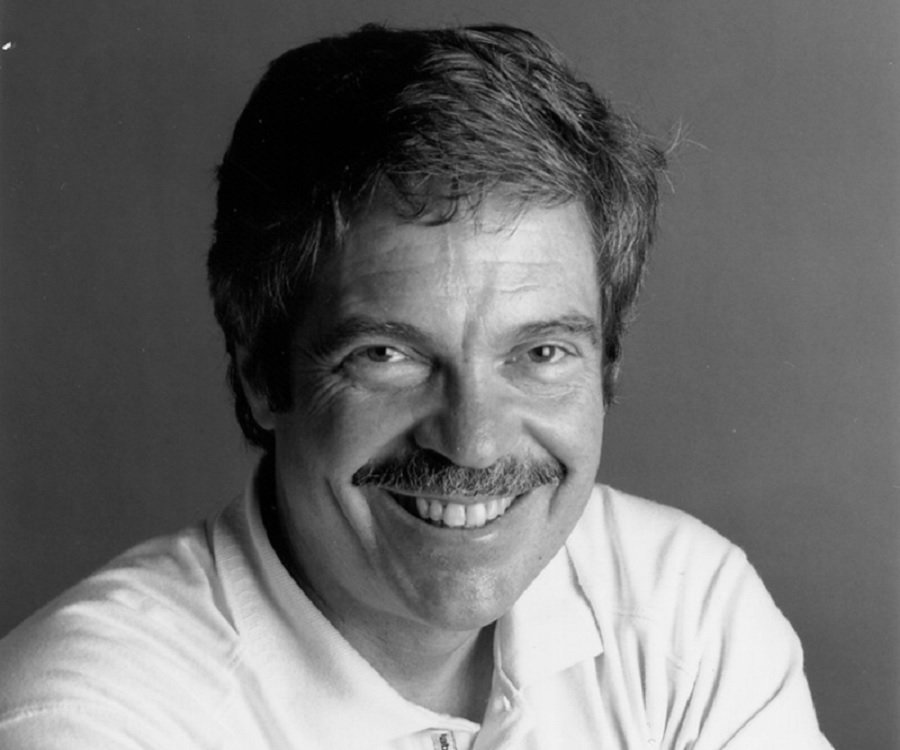
\includegraphics[width=0.25\textwidth]{Smalltalk.jpg}
	\caption{\label{fig:NiklausWirth}Alan Kay.}
\end{wrapfigure}
\emph{Smalltalk} fue creado por Alan Kay, fue el primer lenguaje orientado a objetos. El entorno y el lenguaje son muy maduros, se desarrollo entre 1970 y 1980 en un entorno de investigaci\'on aislado de todo tipo de comercio, por lo que se convirti\'o en una estructura muy bien pensada. Ademas, es uno de los lenguajes orientados a objetos "puros". No hay separaci\'on entre el lenguaje y el ambiente de desarrollo.


\section{Objetos y mensajes}
Todo en Smalltalk es un objeto, incluyendo: 
\begin{itemize}
	\item N\'umeros.
	\item Strings.
	\item Windows.
	\item El compilador.
	\item Partes del ambiente de desarrollo 
\end{itemize}
Los objetos se comunican por el env\'io de mensajes, el mensaje puede retornar un objeto o solamente un mensaje indicando que el proceso finaliz\'o. Ejemplos de expresiones validas para Smalltalk:\newline

\begin{tabular}{c p{2.5cm} p{2cm}}
	Expresi\'on & Objeto recibido & Mensaje\\
	\hline\\
	3 squared & N\'umero entero 3 & squared\\
	\hline\\
	'abc' asUppercase & String 'abc'&asUppercase\\
	\hline\\
	200 factorial & N\'umero entero 200 & factorial \\
	\hline\\
\end{tabular}\newline
Cada mensaje enviado tiene un receptor, nombre del mensaje y cero o mas argumentos, Smalltalk usa tres diferentes formas de sintaxis.

\subsection{Mensajes Unarios}
Esta sintaxis es usada cuando no hay argumentos.
\begin{lstlisting}[language=Smalltalk, caption = {Mensaje enviado en Smalltalk.}][linewidth=5.4cm]

miDepa manager name last

\end{lstlisting}

\begin{lstlisting}[caption = {Mensaje enviado en Java.}][linewidth=5.4cm]

miDepa.manager().name().last()

\end{lstlisting}

El nombre de la variable es miDepa y los dem\'as son nombres de mensajes. 

\subsection{Mensajes Binarios.}
Este mensaje siempre toma exactamente un argumento y el nombre del mensaje puede ser uno o una secuencia de caracteres especiales de los siguientes:
\begin{itemize}
	\item +
	\item *
	\item $<$=
	\item ==
\end{itemize}

\begin{lstlisting}[language=Smalltalk, caption = {Mensaje enviado en Smalltalk.}][linewidth=5.4cm]

x + y 

\end{lstlisting}

\begin{lstlisting}[caption = {Mensaje enviado en Java.}][linewidth=5.4cm]

x.plus(y)

\end{lstlisting}

\subsection{Mensajes Keyword.}
Estos mensajes toman uno o mas argumentos y siempre tendr\'a al menos un car\'acter de dos puntos entre ellos. Con ver el nombre del mensaje se puede notar exactamente cuantos argumentos toma el mensaje con solo contar los caracteres de dos puntos.

\begin{lstlisting}[language=Smalltalk, caption = {Mensaje enviado en Smalltalk.}][linewidth=5.4cm]

x addKey: a value: b

\end{lstlisting}

\begin{lstlisting}[caption = {Mensaje enviado en Java.}][linewidth=5.4cm]

x.addKeyValue(a, b)

\end{lstlisting}
El nombre del mensaje es 'addKey:value:', el car\'acter de dos puntos se usa en el env\'io de estos mensajes ya que es sintacticamente significativo para entender esta sintaxis.
Es importante tener en cuenta que el nombre del mensaje no es un token contiguo. Al ser usado el nombre del mensaje se extiende con expresiones de argumentos intermedios.

\section{Declaraciones de asignaci\'on.}

\begin{lstlisting}[language=Smalltalk, caption = {Sintaxis general de asignaci\'on.}][linewidth=5.4cm]

var := expr

\end{lstlisting}

Siempre se tiene el nombre de la variable a la izquierda del operador que asigna.
Si "var" apunta a un objeto, despu\'es de ser asignado "var" y "expr" van apuntar al mismo objeto.

\section{Conversiones de tipo.}
En Smalltalk solo se tiene una forma de convertir informaci\'on de una representaci\'on a otra, es con el env\'io de mensajes unarios.
\begin{lstlisting}[language=Smalltalk, caption = {Ejemplo de conversiones.}][linewidth=5.4cm]

| d i s |
...
d := i asFloat.
i := d asInteger.
s := i asString.

\end{lstlisting}

\section{Casting.}
Smalltalk tiene un tipo de conversi\'on pero no tiene 'casting', ya que no hay verificaci\'on de tipos, nunca es necesario evitar la verificaci\'on de tipos del compilador.

\section{Clases esenciales.}
En Smalltalk se tienen las siguientes clases que se deben de conocer para empezar a programar.

\subsection{Objeto clase.}
Object es la super clase de todas las clases, por lo que todas las clases pueden heredar sus m\'etodos. Los mas comunes son: 

\subsubsection{printString}
Convierte el objeto que recibe a un objeto string. Se usa cuando se necesita representar un objeto en string para mostrar resultados.

\begin{lstlisting}[language=Smalltalk, caption = {C\'odigo para representar un objeto en string.}][linewidth=5.4cm]

fuelExample
| price |
price := 100.
Dialog warn: 
	'The price is ', price printString

\end{lstlisting}
Esta definici\'on solo retorna el nombre de la clase, si se crea una nueva clase y se quiere convertir a string mas que el nombre, se deber\'ia de cambiar el printString y definir su propio m\'etodo.

\subsubsection{Comparando por igualdad y equivalencia (identidad).}
\begin{tabular}{c p{5cm} p{1cm}}
	S\'imbolo & Funci\'on & Retorna\\
	\hline\\
	= & Verifica si el receptor y argumento son iguales de una forma definida por el programador & true o false\\
	\hline\\
	== & Verifica si el receptor y argumento son uno y el mismo objeto (id\'enticos) & true o false\\
	\hline\\
\end{tabular}
\begin{lstlisting}[language=Smalltalk, caption = {Ejemplo de uso de los comparadores.}][linewidth=5.4cm]

12 = 12.0       "true"
12 == 12.0      "false"

123 = (122 + 1)   "true"
123 = (122 + 1.0)   "true"

123 == (122 + 1)   "true"
123 == (122 + 1.0) "false"

\end{lstlisting}
La comparaci\'on con = es como que solamente tengan el mismo valor y con == es que sean el mismo objeto.
\begin{itemize}
	\item \textasciitilde{}= significa "no iguales".
	\item \textasciitilde{}\textasciitilde{} significa "no identicos".
\end{itemize}
\subsubsection{Proceso de copiado.}
Los m\'etodos de copiado hacen copias del objeto recibido y crean un nuevo objeto del mismo tipo que del recibido. La relaci\'on entre el objeto recibido y el nuevo objeto depende de como est\'an definidos los m\'etodos. Los 2 principales m\'etodos en este protocolo son:
\begin{itemize}
	\item copy: Primero crea una copia superficial del objeto recibido y luego env\'ia un mensaje postCopy al objeto recibido para realizar cualquier otra operaci\'on de copia que se desee.
	\item deepCopy: Copia el objeto recibido y luego de manera recursiva pasa sobre todos los objetos referidos y tambi\'en los copia.
\end{itemize}

\subsection{Clases num\'ericas.}
Estas clases son las mas importantes de utilizar en Smalltalk:
\begin{itemize}
	\item Enteros.
	\item N\'umeros de punto flotante.
	\item Fracciones.
	\item N\'umero fijo de d\'igitos decimales.
	\item N\'umeros complejos.
	\item Metanumeros.
\end{itemize}
Ejemplo de operaciones aritm\'eticas con n\'umeros:

\begin{lstlisting}[language=Smalltalk, caption = {Operaciones a n\'umeros.}][linewidth=5.4cm]

3 + 7 / 3                    
"Mensaje del protocolo aritmetico."
(3 + 7 / 3) asFloat          
"asFloat: del protocolo de conversiones."
(3 + 7 / 3) asFixedPoint: 2  
"asFixedPoint: del protocolo de 
conversiones."
Float pi asRational             
"Tambien del protocolo de conversiones."
15 log                          
"log: es funcion matematica."
0.3 sin                         
"sin: es funcion matematica."
1000 factorial                  
"Protocolo de factorizacion y division."
37 raisedTo: 22                 
"raisedTo: es funcion matematica."
16rF8 + 2r00001000              
"constante se puede obtener 
en base hex, binaria y otras."

\end{lstlisting}

\subsection{Strings}
Un string es una colecci\'on de caracteres indexada que empieza desde el indice 1. Las operaciones a los strings como la concatenaci\'on se da por medio de mensajes.

\begin{lstlisting}[language=Smalltalk, caption = {Ejemplo de mensajes con strings.}][linewidth=5.4cm]

'abcdefg' findString: 'de' startingAt: 1    
"findString: retorna el indice 
o 0 si no lo encuentra"

'abcdefg' size
"size: retorna el tamano del string"

'abcdefg' copyFrom:2 to:4
"Copia el caracter del indice 2 al 4.

\end{lstlisting}

\subsection{Caracteres.}
Cada elemento individual de un string son instancias de la clase Car\'acter. Un car\'acter se puede crear por la conversi\'on del c\'odigo num\'erico, extraer de un string o crear una instancia con el mensaje.

\begin{lstlisting}[language=Smalltalk, caption = {Ejemplo de uso de caracteres.}][linewidth=5.4cm]

Character value:8       
"Caracter del codigo ASCII"
80 asCharacter          
"Caracter del codigo ASCII"
'hola' at:2           
"El segundo elemento del string"
Character cr
"Instancia"
Character esc


\end{lstlisting}

\subsection{S\'imbolos.}
Los s\'imbolos son similares a los strings, pero estas instancias son \'unicas y los strings no lo son. Lo que quiere decir que al crear un nuevo simbolo Smalltalk primero busca que exista otro s\'imbolo con el mismo contenido y devuelve ese objeto existente.
Los s\'imbolos literales se escriben como strings pero con un \# antes. Para s\'imbolos alfanum\'ericos y para selectores binarios se pueden omitir las comillas simples.
\begin{lstlisting}[language=Smalltalk, caption = {Ejemplo de simbolos}][linewidth=3.5cm]

#'abc' = #'abc'
#'abc' == #'abc'    
"retorna true"
"ya que los simbolos son iguales"
\end{lstlisting}

\subsection{Dialogs.}
Contiene muchos mensajes de utilidad para obtener datos como string del usuario.
\begin{lstlisting}[language=Smalltalk, caption = {Ejemplo de uso y tipos de dialogs.}][linewidth=3.5cm]

Dialog request: 'What is your age?'                         
"Retorna string"
Dialog request: 'What is your age?' 
		initialAnswer: '20'     
"Retorna string, tiene por defecto 20"
(Dialog request: 'What is your age?' 
		initialAnswer: '20') asNumber      
"Retorna un numero"
Dialog confirm: 'Are you sure you 
		want to delete the file?'    
"Retorna true o false"
Dialog warn: 'This is a warning'                                
"Retorna nil"
Dialog information: 'This is some
information'                  
"Retorna nil"

\end{lstlisting}

\subsection{Text y ComposedTextView.}
La clase string no tiene informaci\'on como color, tipo de letra, etc. Por lo que se imprime con las propiedades default y si se quiere manipular estas caracter\'isticas se debe de convertir el string al objeto Text.
\begin{lstlisting}[language=Smalltalk, caption = {Ejemplo de uso.}][linewidth=3.5cm]

ComposedTextView open: 
				'abc' asText allBold asValue

\end{lstlisting}
Esto abre una ventana con el texto especificado en negrita.

\subsection{Boolean.}
La clase boolean es abstracta y las clases True y False son subclases, cada una tiene su propia instancia. Principalmente es usado para controlar el flujo de ejecuci\'on, como la ejecuci\'on condicional de un bloque de instrucciones y la repetici\'on condicional.
\begin{lstlisting}[language=Smalltalk, caption = {Ejemplo de uso.}][linewidth=3.5cm]

(4 < 5)                     
"true"
 (4 < 5) ifTrue: 
 	[Transcript clear; show: '4 es menor que 5']                    
ifFalse: 
	[Transcript clear; show: '4 es mayor que 5']

\end{lstlisting}
Los constructores de par\'entesis cuadrados constituyen bloques, la evaluaci\'on de las declaraciones dentro de bloques se retrasan hasta que la definici\'on del mensaje lo solicite expl\'icitamente.

\subsection{Blocks.}
Un bloque es la ejecuci\'on retardada de una secuencia de cero o mas instrucciones, las expresiones dentro del bloque se eval\'uan solo si el programa lo solicita expl\'icitamente.
Son muy importantes y el uso mas com\'un es para la iteraci\'on, ya que se da la evaluaci\'on repetida de una secuencia de enunciados mientras se cumple una condici\'on.

\begin{lstlisting}[language=Smalltalk, caption = {Ejemplo de uso.}][linewidth=3.5cm]

| count |
count := 0.
[count < 100] whileTrue: [count := count + 1].         
"Repite la iteracion hasta que se evalue 
como falso el primer bloque."
Transcript clear; show: count printString          

\end{lstlisting}

\subsection{Colecciones.}
Las clases definen varios tipos de colecciones de objetos y esta es una de las grandes ventajas de Smalltalk. Incluye colecciones con elementos indexados y colecciones desordenadas, cuyos elementos no son accesados por un indice. La mayor\'ia de colecciones son din\'amicas ya que su tama\~no puede ser cambiado en tiempo de ejecuci\'on pero existen un par que tienen tama\~no fijo. Las colecciones que son indexadas empiezan con el indice 1. Ademas, la mayor\'ia de colecciones aceptan cualquier objeto pero un par solo aceptan cierto tipo de objetos.

\subsubsection{Collection.}
Es una super clase abstracta de todas las colecciones. No tiene instancias ya que su prop\'osito es definir todo lo que comparten la mayor\'ia de las colecciones.

\subsubsection{Array.}
Es indexado y el primer indice es 1, los elementos no pueden ser agregados o eliminados, solo sus valores pueden cambiar.
\begin{lstlisting}[ caption = {Array creado como literal.}][linewidth=3.5cm]

#(1 2 3 $a $b $c 'abc' 3.14 #symbol true)          

\end{lstlisting}
\begin{lstlisting}[language=Smalltalk, caption = {Array vacio con un tama\~no predefinido.}][linewidth=3.5cm]

|a|

a := Array new:100.
a at:50 put:'fifty'.
a inspect.         

\end{lstlisting}
\begin{lstlisting}[language=Smalltalk, caption = {Los elementos del array pueden ser arrays.}][linewidth=3.5cm]

#(
(1 'one')
(2 'two')
(3 'three')
)        

\end{lstlisting}
\subsubsection{OrderedCollection.}
Similar al array pero es de tama\~no variable. Los usos son algo diferentes.
\begin{lstlisting}[language=Smalltalk, caption = {Uso de OrderedCollection.}][linewidth=3.5cm]

|o|

o := OrderedCollection new.
o add:'one'.
o add:'two'.
o add:'three'.
o inspect.        

\end{lstlisting}
\subsubsection{SortedCollection.}
Es una subclase de OrderedCollection que ordena sus elementos usando un bloque de clasificaci\'on. Por defecto usa sort block.
\begin{lstlisting}[language=Smalltalk, caption = {Bloque para ordenar elementos.}][linewidth=3.5cm]

[:elemento1 :elemento2 | elemento1 < elemento2]
        
\end{lstlisting}
\subsubsection{Set.}
Es una colecci\'on desordenada, sin indice y elimina autom\'aticamente los elementos duplicados.
\begin{lstlisting}[language=Smalltalk, caption = {Ejemplo para convertir a un Set.}][linewidth=3.5cm]

#(1 1 2 3 3 2.0) asSet

\end{lstlisting}
\subsubsection{IdentitySet.}
Es como el Set, pero usa identidad en lugar de igualdad para comprobar la duplicaci\'on, la verificaci\'on de identidad es mas r\'apida que la de igualdad.
\begin{lstlisting}[language=Smalltalk, caption = {Ejemplo para convertir a IdentitySet.}][linewidth=3.5cm]

#(1 1 1 2 2 2 3 3 3 2.0) asIdentitySet

\end{lstlisting}

\subsubsection{Dictionary.}
Es un conjunto de asociaciones, una asociaci\'on es un par con clave-valor y se crea con el mensaje binario $->$.
\begin{lstlisting}[language=Smalltalk, caption = {Ejemplo para agregar a un diccionario.}][linewidth=3.5cm]

Dictionary new
add: 'CRT' -> 'Cathode Ray Tube';
add: 'SSI' -> 'Small Scale Integration';
yourself

\end{lstlisting}

\begin{lstlisting}[language=Smalltalk, caption = {Ejemplo para actualizar diccionario.}][linewidth=3.5cm]

Dictionary new
add: 'key1' -> 'old value';
add: 'key1' -> 'new value';
yourself

\end{lstlisting}

\subsubsection{IdentityDictionary.}
Es similar al diccionario, pero usa la identidad para probar la duplicaci\'on de elementos. ademas es mas eficiente que el diccionario ya que las pruebas de identidad son mucho mas r\'apidas que las pruebas de igualdad. 
\begin{lstlisting}[language=Smalltalk, caption = {Ejemplo con 2 entradas en la misma llave.}][linewidth=3.5cm]

IdentityDictionary new
add: 'key1' -> 'old value';
add: 'key1' -> 'new value';
yourself 

\end{lstlisting}

\subsubsection{Bag.}
Es como el Set, pero la bolsa sabe cuantas apariciones de un elemento se presentan.
\begin{lstlisting}[language=Smalltalk, caption = {Ejemplo de Bag.}][linewidth=3.5cm]

#(1 1 1 2 2 2 3 3 3) asBag

\end{lstlisting}

\subsubsection{Interval.}
Es una representaci\'on compacta de una progresi\'on aritm\'etica, es una secuencia de n\'umeros igualmente espaciados.
\begin{lstlisting}[language=Smalltalk, caption = {Representa una secuencia 3, 4, 5, 6, 7, 8, 9.}][linewidth=3.5cm]

Interval from: 3 to: 9

\end{lstlisting}

\section{Declaraciones de flujo de control.}
Cada una de las declaraciones de flujo de control se hace usando un mensaje. Ejemplo: La instrucci\'on "if" usa el mensaje "ifTrue: ifFalse:".

\subsection{La declaraci\'on \emph{If}}
La instrucci\'on if inicia con la expresi\'on booleana. Los par\'entesis cuadrados se requieren, incluso si solo hay una declaraci\'on. Ambos argumentos para el m\'etodo 'ifTrue: ifFalse:' deben de ser bloques.

\begin{lstlisting}[language=Smalltalk, caption = {Sintaxis de un If}][linewidth=5.0cm]

(x < y) ifTrue: [
max := y.
i := j
] ifFalse: [
max := x.
i := k
]

\end{lstlisting}
Hay solo 3 tipos diferentes de mensajes:
\begin{itemize}
	\item ifTrue:ifFalse:
	\item ifTrue:
	\item ifFalse:
\end{itemize}

\subsection{La declaraci\'on \emph{While}}
La expresi\'on debe de estar entre par\'entesis, ya que debe de evaluarse cada vez que hace el ciclo 
\begin{lstlisting}[language=Smalltalk, caption = {Ejemplo de un ciclo "while".}][linewidth=5.0cm]

[i < 100] whileTrue: [
sum := sum + i.
i := i + 1
]

\end{lstlisting}

\subsection{La declaraci\'on de \emph{For}}

\begin{lstlisting}[language=Smalltalk, caption = {Ejemplo de un ciclo "for".}][linewidth=5.0cm]

1 to: n do: [ :i |
sum := sum + i.
] 

\end{lstlisting}
El cuerpo del ciclo se ejecuta iterativamente con valores incrementados en 1 de 'i', en el rango de 1 a n. La variable 'i' es local al cuerpo del ciclo y no puede ser accesible desde otra parte.

\subsection{La declaraci\'on de \emph{Return}}
Se usa el car\'acter \char`\^ para retornar un valor

\begin{lstlisting}[ caption = {Comparaci\'on de return}][linewidth=5.0cm]

 ^ i+6         "Smalltalk"
 
 return i+6;   //Java

\end{lstlisting}

\subsection{Comentarios en el c\'odigo}
Los comentarios se encierran en comillas dobles. Los comentarios son mas f\'aciles de leer junto al c\'odigo. Ademas, al hacer comentarios se ven integrados al c\'odigo y es mas f\'acil entenderlo que es un documento aparte, aunque los comentarios est\'an integrados al c\'odigo no se destacan tanto en Smalltalk.
\subsection{Comparaci\'on de nombres predefinidos con Java.}
Son muy peque\~nas las diferencias en la sintaxis, tambi\'en hay varios nombres predefinidos que son identificadores de objetos espec\'ificos.\newline\newline
\begin{tabular}{c p{2cm} p{10cm}}
	Smalltalk & Java\\
	\hline
	$1234$ & $1234$\\
	$11.34$ & $11.34$\\
	\$a & $'a'$\\
	$'hello'$ & $"hello"$\\
	$nil$ & $null$\\
	$true$ & $true$\\
	$false$ & $false$\\
	$self$ & $this$\\
	$super$ & $super$\\
	\hline 
\end{tabular}

\subsection{Variables de clases.}
Es una variable que puede ser accesada globalmente en la clase. Solo hay una copia de cada variable y es compartida por todas las instancias, se puede acceder a una variable de clase desde cualquier parte del c\'odigo mientras se este dentro de la clase, sin necesidad de una referencia a alguna instancia en especifico.
Por ejemplo, se tiene la clase Persona, se necesita un contador de las instancias de Persona, entonces solo se agrega a la clase Persona una variable llamada PersonaCount y cada ves que se cree una instancia, se aumenta el contador en uno.
\begin{lstlisting}[language=Smalltalk, caption = {Ejemplo de contador de la clase Persona.}][linewidth=5.0cm]

PersonaCount := PersonaCount + 1

\end{lstlisting}

\subsection{M\'etodos de clases.}
M\'etodo que es parte de una clase, pero no es invocado en una instancia particular, ademas se pueden invocar antes de que se hayan creado instancias.
Por ejemplo, se tiene la clase Persona con una variable que es el total de instancias de la clase Persona, se crea un m\'etodo de la clase llamado 'printStatics' para imprimir el valor de todas las variables de la clase.
Para invocar un m\'etodo de una clase, un mensaje es enviado a la misma clase.
\begin{lstlisting}[language=Smalltalk, caption = {Ejemplo de metodo de la clase Persona}][linewidth=5.0cm]

Person printStatistics

\end{lstlisting}

\subsection{Creaci\'on de objetos.}
Toda clase se representa por un objeto. Ejemplo: La clase Estudiante es representada por el objeto Estudiante. Al invocar un m\'etodo de la clase, se invoca un m\'etodo de la instancia por el env\'io de mensajes a una instancia de la clase.
\begin{lstlisting}[language=Smalltalk, caption = {Ejemplo para crear una instancia de la clase Persona.}][linewidth=5.0cm]

p := Persona new

\end{lstlisting}
Normalmente, el m\'etodo 'new' es heredado de una implementaci\'on en la clase 'Object', creara un nuevo objeto y lo retornara. Se puede sobrescribir el m\'etodo 'new', por ejemplo para incrementar la variable contador de la clase Persona. As\'i, le damos diferentes valores iniciales ya que las variables y campos, son inicializados en 'nil'.

\subsection{Constructores.}
No existen en Smalltalk, pero brinda la misma funcionalidad sin nueva sem\'antica o sintaxis. En Java o C++ los constructores inicializan nuevas instancias y tambi\'en agregan valores iniciales. En Smalltalk tambi\'en se modifican algunas variables est\'aticas como 'PersonaCount' dentro del constructor, por ejemplo se puede crear un m\'etodo de clase que tome dos par\'ametros.
\begin{lstlisting}[language=Smalltalk, caption = {Ejemplo para crear una instancia de la clase Persona.}][linewidth=5.0cm]

p := Person newNombre: 'John' edad: 15

\end{lstlisting}
En este ejemplo el m\'etodo de la clase hereda del m\'etodo 'new' para crear el objeto y luego modifica unos campos y tambi\'en actualiza la variable de la clase.

\subsection{Operadores matem\'aticos.}
\begin{tabular}{c p{4cm} p{1cm}}
	Operador & Significado\\
	\hline\\
	$+ , - $ & Suma, Resta \\
	$* , /$ & Multiplicaci\'on,  Divisi\'on\\
	$bitAnd , bitOr , bitXor$ & Operadores bitwise\\
	$bitInvert$ & Invertir bitwise\\
	$bitShift$ & Operadores bitwise \\
	$raisedTo$ & Exponente\\
	$log: 10$ & Logaritmo base 10\\
	$ln$ & Logaritmo natural\\
	$rem$ & Modulo con negativos\\
	\textbackslash{}\textbackslash{} & Modulo valor abs\\
	$-$ & Negacion\\
	$1000.0, 1E3$ & Sintaxis punto flotante\\
	$2r1$ & Sintaxis enteros con base 2\\
	$100$ & Sintaxis de numero entero\\
	$sqrt $ & Ra\'iz cuadrada\\
	$raisedTo$ & Exponente\\
	$exp, abs$ & Exponente e, valor absoluto\\
	$sin, cos, tan$ & Trigonometria b\'asica\\
	$arcSin, arcCos, arcTan$ & Trigonometria inversa\\
	$rounded, floor$ & Redondear\\
	$Float, Double$ & Nombre de tipos de punto flotante\\
	$Fraction, FixedPoint$ & Nombre de tipos de punto flotante\\
	$Integer, SmallInteger$ & Nombre de tipos enteros\\
	$LargeInteger$ & Nombre de tipos enteros\\	
	\hline
\end{tabular}

\subsection{Operadores Booleanos}
\begin{tabular}{c p{6cm} p{15cm}}
	Operador & Significado\\
	\hline\hline
	$and$ & and l\'ogico (short circuit)\\\hline
	$or$ & or l\'ogico (short circuit)\\\hline
	$not$ & Negaci\'on l\'ogica\\\hline
	$false$ & Valor falso\\\hline
	$true$ & Valor verdadero\\\hline
	$Boolean$ & Nombre del tipo\\\hline
	$|$ & or l\'ogico (eval\'ua ambos argumentos)\\\hline
	\& & and l\'ogico (eval\'ua ambos argumentos)\\
	\hline 
\end{tabular}

\section{Herencia.}
Las clases est\'an relacionadas, la clase Object es la \'unica que no tiene una superclase, el resto de clases tienen exactamente una superclase y tiene todas las variables de instancia de su superclase y comprende todos sus mensajes.
Si A es superclase de B y B es la superclase de C, C hereda de B incluyendo todo lo que B hereda de A, por lo que C hereda todo lo de B y A. Es transitiva. Entonces todas las clases heredan todo el comportamiento de la clase Object.
\begin{lstlisting}[language=Smalltalk, caption = {Ejemplo para conocer la superclase de una clase.}][linewidth=5.0cm]

Fraction superclass

\end{lstlisting}

\section{Self y Super.}
'Self' se refiere al receptor en si, es significado es id\'entico al 'this' de Java. 'Super' y 'self' se refieren al mismo objeto, el receptor del m\'etodo, la diferencia es que 'super' busca desde la superclase del m\'etodo que usa 'super'.
\begin{lstlisting}[language=Smalltalk, caption = {Ejemplo del "Self".}][linewidth=5.0cm]

self computeTaxes.
phoneBook at: self put: i

\end{lstlisting}


\section{Accesando campos de objetos.}
En Smalltalk, los campos de un objeto no se pueden acceder desde fuera de la clase. Ademas, todos los campos son privados, entonces todos los accesos externos deben de darse por medio de m\'etodos, que se conocen como m\'etodos de acceso.
\begin{lstlisting}[caption = {Ejemplo de m\'etodo de acceso al campo "name" de una clase.}][linewidth=5.0cm]

name
	"Retorna."
	^ name

name: str
	"Actualiza."
	name := str

\end{lstlisting}

\section{Caracter\'isticas}
\begin{itemize}
	\item Interacci\'on entre objetos mediante el env\'io de mensajes.
	\item Se da herencia simple y con ra\'iz com\'un.
	\item Garbage collector.
	\item El c\'odigo fuente es parte del entorno, por lo que es disponible para su extenci\'on, modificaci\'on y estudio.
	\item Es fuertemente tipado, es decir un objeto no puede ejecutar un mensaje que no fue programado.
	\item Es dinamicamente tipado, es decir al evaluar un mensaje, encuentra la definici\'on en tiempo de ejecuci\'on.
\end{itemize}

\section{Ventajas}
\begin{itemize}
	\item Las reglas del lenguaje son simples.
	\item El ambiente de desarrollo es muy poderoso.
	\item El c\'odigo que escribe un programador con experiencia en Smalltalk es legible y muy compacto.
	\item Es un lenguaje muy flexible y las aplicaciones son muy extensibles.
	\item No se necesita el "casting" de tipos.
\end{itemize}


\section{Desventajas}
\begin{itemize}
	\item La sintaxis es distinta a otros lenguajes, ya que sigue el paradigma de envio de mensajes.
	\item Algunos entornos no incorporan manejo de excepciones.
	\item No es estandarizado, es decir se presentan muchas diferencias entre versiones.
\end{itemize}

\begin{thebibliography}{3}
	
	\bibitem{Smalltalk}
	T.~Budd. 1987. \emph{A Little Smalltalk.}Recuperado de http://sdmeta.gforge.inria.fr/FreeBooks/
	LittleSmalltalk/ALittleSmalltalk.pdf
	
	\bibitem{Smalltalk1}
	W.~Lalonde. 1994. \emph{Discovering Smalltalk.} Object Technology Series. Recuperado de https://books.google.co.cr/books/about/Discovering\_Smalltalk.
	html?id=t4RQAAAAMAAJ\&redir\_esc=y
		
	\bibitem{Smalltalk2}
	S.~Lewis. 1995. \emph{The Art and Science of Smalltalk.} Textbook Binding. Recuperado de http://sdmeta.gforge.inria.fr/FreeBooks/Art/
	artAdded174186187Final.pdf
	
	\bibitem{Smalltalk3}
	J.~Pletzke. 1985. \emph{Advanced Smalltalk.} Computer Publishing. John Wiley \& Sons, Inc.
	
	\bibitem{Smalltalk4}
	D, Gomez. 2006. \emph{Libro de programaci\'on con Smalltalk}. Recuperado de http://diegogomezdeck.blogspot.com/2006/02/libro-programando-con-smalltalk.html
	
\end{thebibliography}

\end{document}


